\documentclass{article}
\usepackage{../assignment_preamble}

\title{Homework 3}
\author{Ravi Kini}
\date{October 31, 2025}

\begin{document}

\maketitle

\problem{}
\begin{align*}
    H_v = I - 2\frac{vv^T}{v^T v}
\end{align*}\
\subproblem{(a)}
Taking the transpose of $H_v$:
\begin{align*}
    H_v^T & = I^T - 2\frac{{(vv^T)}^T}{v^T v} \\
    & = I - 2\frac{{vv^T}^T}{v^T v} = H_v \\
\end{align*}
Therefore $H_v$ is symmetric.
\subproblem{(b)}
Finding $H_{\alpha v}$:
\begin{align*}
    H_{\alpha v} & = I - 2\frac{(\alpha v){(\alpha v)}^T}{{(\alpha v)}^T(\alpha v)} \\
    & = I - 2\frac{\alpha^2(vv^T)}{\alpha^2(vv^T)} \\
    & = I - 2\frac{vv^T}{v^T v} = H_v
\end{align*}
Therefore $H_v$ is independent of the scaling of $\alpha$.
\subproblem{(c)}
Finding $H_v^2$:
\begin{align*}
    H_v^2 & = {\left(I - 2\frac{vv^T}{v^T v}\right)}^2 \\
    & = I - 4\frac{vv^T}{v^T v} + 4{\left(\frac{vv^T}{v^T v}\right)}^2 \\
    & = I - 4\frac{vv^T}{v^T v} + 4\frac{v(v^T v)v^T}{{(v^T v)}^2} \\
    & = I - 4\frac{vv^T}{v^T v} + 4\frac{vv^T}{v^T v} \\
    & = I
\end{align*}
Therefore $H_v$ is involutary.
\subproblem{(d)}
Since $H_v$ is involutary, $H_v^{-1} = H_v$.

\clearpage
\problem{}
Let $x, y \in \mathbb{R}^n$ such that $x \neq y$ and $||x||_2 = ||y||_2$. Then:
\begin{align*}
    H_v x & = \left(I - 2\frac{vv^T}{v^T v} \right)x 
    y = x - 2v\frac{v^T x}{v^T v} \\
    2v\frac{v^T x}{v^T v} & = x - y \\
    v & = (x - y) \frac{v^T v}{2v^T x} \\
\end{align*}
Since scaling $v$ should not affect the formula, we choose $v = x - y$.

\clearpage
\problem{}
\begin{align*}
    A = \begin{bmatrix}
        1 & 1 & 1 \\
        0 & 1 & 1 \\
        0 & 1 & 0
    \end{bmatrix}
\end{align*}
The first column $a_1 = e_1$ already, so we move on to the second column and focus on the $2 \times 2$ submatrix, letting $R_1 = A, Q_1 = I$. The second column of $A$ has norm $\sqrt{1^2 + 1^2} = \sqrt{2}$, so we let $v = a_2 - \sqrt{2}e_2 = {(1-\sqrt{2}, 1)}^T$. This yields the elimination matrix:
\begin{align*}
    H_v & = \begin{bmatrix}
        1 & 0 \\
        0 & 1 \\
    \end{bmatrix} - \frac{2}{4 - 2\sqrt{2}}\begin{bmatrix}
        3 - 2\sqrt{2} & 1 - \sqrt{2} \\
        1 - \sqrt{2} & 1 \\
    \end{bmatrix} \\
    & = \begin{bmatrix}
        \sqrt{2}/2 & \sqrt{2}/2 \\
        \sqrt{2}/2 & -\sqrt{2}/2 \\
    \end{bmatrix} \\
\end{align*}
Then, expanding to $3 \times 3$:
\begin{align*}
    R_2 & = H_v R_1 = \begin{bmatrix}
        1 & 1 & 1 \\
        0 & \sqrt{2} & \sqrt{2}/2 \\
        0 & 0 & \sqrt{2}/2
    \end{bmatrix}\\
    Q_2 & = \begin{bmatrix}
        1 & 0 & 0 \\
        0 & \sqrt{2}/2 & \sqrt{2}/2 \\
        0 & \sqrt{2}/2 & -\sqrt{2}/2 \\
    \end{bmatrix} \\
\end{align*}
Since $R$ is now upper triangular, we have:
\begin{align*}
    A & = \begin{bmatrix}
        1 & 0 & 0 \\
        0 & \sqrt{2}/2 & \sqrt{2}/2 \\
        0 & \sqrt{2}/2 & -\sqrt{2}/2 \\
    \end{bmatrix}\begin{bmatrix}
        1 & 1 & 1 \\
        0 & \sqrt{2} & \sqrt{2}/2 \\
        0 & 0 & \sqrt{2}/2
    \end{bmatrix}
\end{align*}
This is the same factorization that is found by using the Gram-Schmidt method.

\clearpage
\problem{}
If $a \in \mathbb{R}^n$ is treated as a $n \times 1$ matrix $A$, for the full QR factorization, $Q$ must be a $n \times n$ matrix and $R$ must a $n \times 1$ upper triangular matrix. The columns of $Q$ will be the $n$ vectors found using the Gram-Schmidt method; we define $q_i = e_i - \sum_{j=1}^{i - 1} \mathrm{proj}_{q_j}(e_i)$, with $q_0 = a/||a||_2$. Let $q_1', \ldots q_n'$ be the first $n$ nonzero vectors produced by this method. $R$ then has $||a||_2$ as its first entry, and all other entries be zero.
\begin{align*}
    a = A & = \begin{bmatrix}
        a/||a||_2 & q_2' & \cdots & q_n'
    \end{bmatrix}\begin{bmatrix}
        ||a||_2 \\
        0 \\
        \vdots \\
        0 \\
    \end{bmatrix}
\end{align*}
For the reduced QR factorization, we look only at the first entry of $R$, as all following are zero, and correspondingly, the first column of $Q$:
\begin{align*}
    a = A & = \begin{bmatrix}
        a/||a||_2
    \end{bmatrix}\begin{bmatrix}
        ||a||_2 \\
    \end{bmatrix}
\end{align*}

\clearpage
\problem{}
\begin{align*}
    Q = A{(L^T)}^{-1}
\end{align*}
\subproblem{}
Taking the transpose of $Q$:
\begin{align*}
    Q^T & = {(A{(L^T)}^{-1})}^{-1} \\
    & = L^{-1} A^T
\end{align*}
Then:
\begin{align*}
    QQ^T & = A{(L^T)}^{-1}L^{-1} A^T \\
    &  = A{(LL^T)}^{-1}A^T \\
    &  = A{(A^T A)}^{-1}A^T \\
    &  = AA^{-1}{(A^T)}^{-1}A^T \\
    & = I
\end{align*}
Therefore $Q$ is an orthonormal matrix.
\subproblem{}
If $LL^T$ is the Cholesky factorization of $A^T A$, then in the QR factorization of $A$, $Q = A(L^T)^{-1}$ and $R = L^T$.

\clearpage
\problem{}
We seek to minimize:
\begin{align*}
    \phi(\alpha, \beta) = \sum_{i=1}^m {((a + \beta t_i) - \sqrt{t_i})}^2
\end{align*}
where $t_i = \frac{1}{4} + \frac{3}{4}\frac{i - 1}{m - 1}$. We solve the least squares problem where:
\begin{align*}
    A & = \begin{bmatrix}
        1 & t_1 \\ 1 & t_2 \\ \vdots & \vdots \\ 1 & t_m
    \end{bmatrix} \\
    x & = \begin{bmatrix}
        \alpha \\ \beta
    \end{bmatrix} \\
    b & = \begin{bmatrix}
        \sqrt{t_1} \\
        \sqrt{t_2} \\
        \vdots \\
        \sqrt{t_m}
    \end{bmatrix}
\end{align*}
We seek to solve the normal equation:
\begin{align*}
    A^T A x = A^T b
\end{align*}
This can be done using the following program:
\begin{lstlisting}[language=Python]
def transpose(A):
    A_r, A_c = len(A), len(A[0])
    A_T = [[A[i][j] for i in range(A_r)] for j in range(A_c)]
    return A_T
    
def multiply(A, B):
    A_r, A_c = len(A), len(A[0])
    B_r, B_c = len(B), len(B[0])
    AB = [[0 for _ in range(B_c)] for __ in range(A_r)]
    for i in range(A_r):
        for j in range(B_c):
            for k in range(A_c):
                AB[i][j] += A[i][k] * B[k][j]
    return AB

def inverse(A):
    A_ = A.copy()
    A_rc = len(A_)
    for i in range(A_rc):
        A_[i].extend([int(i == j) for j in range(A_rc)])
    for i in range(A_rc - 1, 0, -1):
        if A_[i - 1][0] < A_[i][0]:
            A_[i - 1], A_[i] = A_[i], A_[i - 1]
    for i in range(A_rc):
        for j in range(A_rc):
            if j != i:
                tmp = A_[j][i] / A_[i][i]
                for k in range(2 * A_rc):
                    A_[j][k] -= A_[i][k] * tmp
    for i in range(A_rc):
        tmp = A_[i][i]
        for j in range(2 * A_rc):
            A_[i][j] = A_[i][j] / tmp
    return [A_[i][A_rc:] for i in range(A_rc)]
    
m = 4

t = lambda i: 1/4 + 3/4 * (i - 1) / (m - 1)

A = [[1, t(i)] for i in range(1, m + 1)]
b = [[t(i) ** 0.5] for i in range(1, m + 1)]

x = multiply(inverse(multiply(transpose(A), A)), multiply(transpose(A), b))
print(x)
\end{lstlisting}
Plotting the function and the computed line of best fit:
\begin{center}
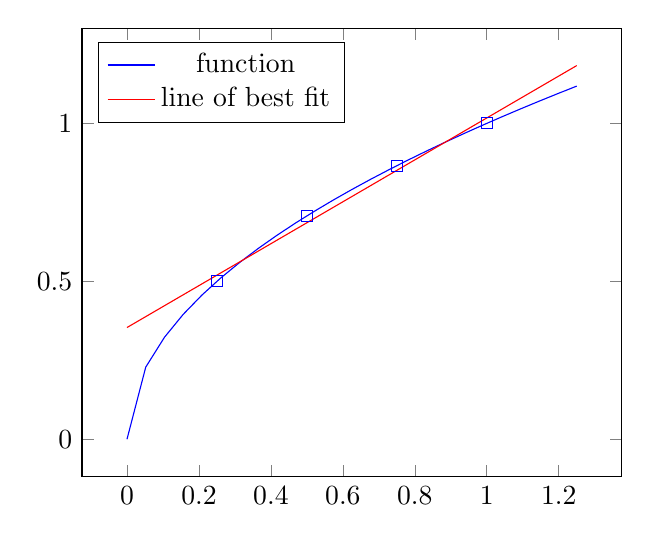
\begin{tikzpicture}
\begin{axis}[legend pos=north west]
\addlegendentry{function}
\addplot[color=blue,domain=0:1.25]{sqrt(x)};
\addlegendentry{line of best fit}
\addplot[color=red,domain=0:1.25]{0.35355339059327306 + 0.6635674490391574 * x};
\addplot[color=blue, mark=square,only marks]
coordinates {
(0.25,0.5)(0.5,0.707)(0.75,0.866)(1.0,1.0)
};
\end{axis}
\end{tikzpicture}
\end{center}

\clearpage
\problem{}
We solve the least squares problem where:
\begin{align*}
    A & = \begin{bmatrix}
        1 & -1 & 0 & 0 \\
        -1 & 0 & 1 & 0 \\
        1 & 0 & 0 & -1 \\
        0 & 0 & 1 & -1 \\
        0 & 1 & 0 & -1 \\
        1 & 1 & 1 & 1 \\
    \end{bmatrix} \\
    x & = \begin{bmatrix}
        r_1 \\ r_2 \\ r_3 \\ r_4
    \end{bmatrix} \\
    b & = \begin{bmatrix}
        4 \\ 9 \\ 6 \\ 3 \\ 7 \\ 100
    \end{bmatrix}
\end{align*}
We seek to solve the normal equation:
\begin{align*}
    A^T A x = A^T b
\end{align*}
This can be done using the following program:
\begin{lstlisting}[language=Python]
def transpose(A):
    A_r, A_c = len(A), len(A[0])
    A_T = [[A[i][j] for i in range(A_r)] for j in range(A_c)]
    return A_T
    
def multiply(A, B):
    A_r, A_c = len(A), len(A[0])
    B_r, B_c = len(B), len(B[0])
    AB = [[0 for _ in range(B_c)] for __ in range(A_r)]
    for i in range(A_r):
        for j in range(B_c):
            for k in range(A_c):
                AB[i][j] += A[i][k] * B[k][j]
    return AB

def inverse(A):
    A_ = A.copy()
    A_rc = len(A_)
    for i in range(A_rc):
        A_[i].extend([int(i == j) for j in range(A_rc)])
    for i in range(A_rc - 1, 0, -1):
        if A_[i - 1][0] < A_[i][0]:
            A_[i - 1], A_[i] = A_[i], A_[i - 1]
    for i in range(A_rc):
        for j in range(A_rc):
            if j != i:
                tmp = A_[j][i] / A_[i][i]
                for k in range(2 * A_rc):
                    A_[j][k] -= A_[i][k] * tmp
    for i in range(A_rc):
        tmp = A_[i][i]
        for j in range(2 * A_rc):
            A_[i][j] = A_[i][j] / tmp
    return [A_[i][A_rc:] for i in range(A_rc)]
    
A = [[1, -1, 0, 0], [-1, 0, 1, 0], [1, 0, 0, -1], [0, 0, 1, -1], [0, 1, 0, -1], [1, 1, 1, 1]]
b = [[4], [9], [6], [3], [7], [100]]

x = multiply(inverse(multiply(transpose(A), A)), multiply(transpose(A), b))
print(x)
\end{lstlisting}
This yields:
\begin{align*}
    x = \begin{bmatrix}
        25.25 \\ 24.625 \\ 29.125 \\ 21.0
    \end{bmatrix}
\end{align*}
We rank Team 3 first, Team 1 second, Team 2 third, and Team 4 fourth.
\end{document}